\documentclass{article}
\usepackage[T1]{fontenc}
\usepackage[utf8]{inputenc}
\usepackage{lmodern}
\usepackage[T1]{fontenc}
\usepackage[utf8]{inputenc}
\usepackage{lmodern}
\usepackage[T1]{fontenc}
\usepackage[utf8]{inputenc}
\usepackage{lmodern}
\usepackage[tmargin=1cm,lmargin=1cm]{geometry}
\usepackage{tikz}
\usepackage{pgfplots}
\pgfplotsset{compat=newest}
\usepackage{pgfplots}


\begin{document}
\section{Series: h}
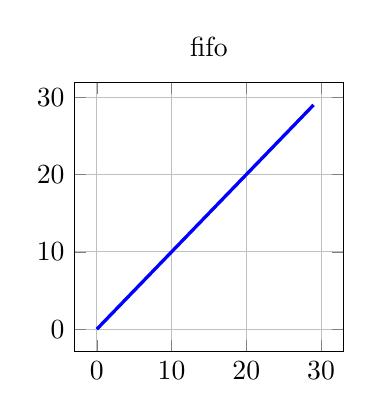
\begin{tikzpicture}
\begin{axis}[title=fifo, height=5cm, width=5cm, grid=major, xmin=({-}3.0), xmax=(33.0), ymin=({-}2.9), ymax=(31.9)]
\addplot[very thick,color=blue] coordinates { (0,0) (1,1) (2,2) (3,3) (4,4) (5,5) (6,6) (7,7) (8,8) (9,9) (10,10) (11,11) (12,12) (13,13) (14,14) (15,15) (16,16) (17,17) (18,18) (19,19) (20,20) (21,21) (22,22) (23,23) (24,24) (25,25) (26,26) (27,27) (28,28) (29,29)
};


\end{axis}
\end{tikzpicture}
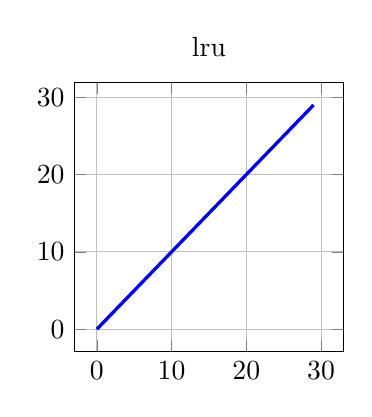
\begin{tikzpicture}
\begin{axis}[title=lru, height=5cm, width=5cm, grid=major, xmin=({-}3.0), xmax=(33.0), ymin=({-}2.9), ymax=(31.9)]
\addplot[very thick,color=blue] coordinates { (0,0) (1,1) (2,2) (3,3) (4,4) (5,5) (6,6) (7,7) (8,8) (9,9) (10,10) (11,11) (12,12) (13,13) (14,14) (15,15) (16,16) (17,17) (18,18) (19,19) (20,20) (21,21) (22,22) (23,23) (24,24) (25,25) (26,26) (27,27) (28,28) (29,29)
};


\end{axis}
\end{tikzpicture}
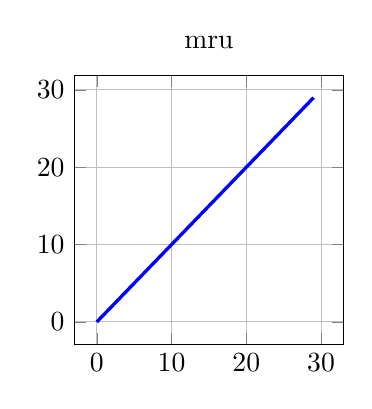
\begin{tikzpicture}
\begin{axis}[title=mru, height=5cm, width=5cm, grid=major, xmin=({-}3.0), xmax=(33.0), ymin=({-}2.9), ymax=(31.9)]
\addplot[very thick,color=blue] coordinates { (0,0) (1,1) (2,2) (3,3) (4,4) (5,5) (6,6) (7,7) (8,8) (9,9) (10,10) (11,11) (12,12) (13,13) (14,14) (15,15) (16,16) (17,17) (18,18) (19,19) (20,20) (21,21) (22,22) (23,23) (24,24) (25,25) (26,26) (27,27) (28,28) (29,29)
};


\end{axis}
\end{tikzpicture}
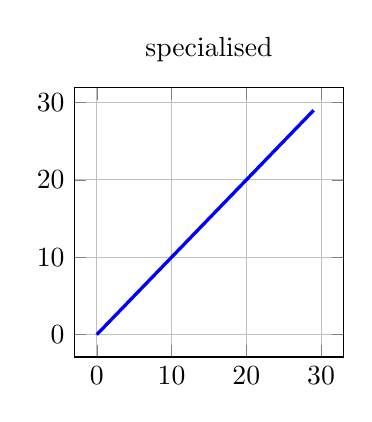
\begin{tikzpicture}
\begin{axis}[title=specialised, height=5cm, width=5cm, grid=major, xmin=({-}3.0), xmax=(33.0), ymin=({-}2.9), ymax=(31.9)]
\addplot[very thick,color=blue] coordinates { (0,0) (1,1) (2,2) (3,3) (4,4) (5,5) (6,6) (7,7) (8,8) (9,9) (10,10) (11,11) (12,12) (13,13) (14,14) (15,15) (16,16) (17,17) (18,18) (19,19) (20,20) (21,21) (22,22) (23,23) (24,24) (25,25) (26,26) (27,27) (28,28) (29,29)
};


\end{axis}
\end{tikzpicture}


\section{Series: math.log10(h / h + ncm)}
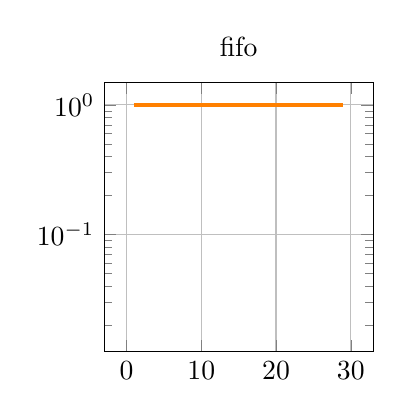
\begin{tikzpicture}
\begin{axis}[ymode=log, title=fifo, height=5cm, width=5cm, grid=major, xmin=({-}3.0), xmax=(33.0), ymin=(0.012427), ymax=(1.490182)]
\addplot[very thick,color=orange] coordinates { (1,1.0) (2,1.0) (3,1.0) (4,1.0) (5,1.0) (6,1.0) (7,1.0) (8,1.0) (9,1.0) (10,1.0) (11,1.0) (12,1.0) (13,1.0) (14,1.0) (15,1.0) (16,1.0) (17,1.0) (18,1.0) (19,1.0) (20,1.0) (21,1.0) (22,1.0) (23,1.0) (24,1.0) (25,1.0) (26,1.0) (27,1.0) (28,1.0) (29,1.0)
};


\end{axis}
\end{tikzpicture}
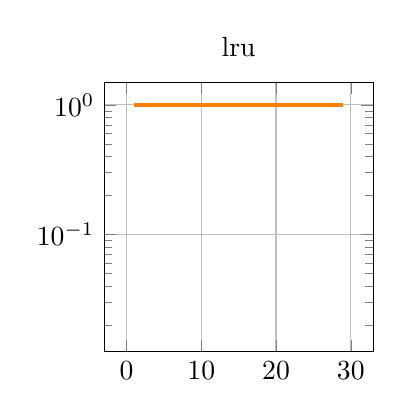
\begin{tikzpicture}
\begin{axis}[ymode=log, title=lru, height=5cm, width=5cm, grid=major, xmin=({-}3.0), xmax=(33.0), ymin=(0.012427), ymax=(1.490182)]
\addplot[very thick,color=orange] coordinates { (1,1.0) (2,1.0) (3,1.0) (4,1.0) (5,1.0) (6,1.0) (7,1.0) (8,1.0) (9,1.0) (10,1.0) (11,1.0) (12,1.0) (13,1.0) (14,1.0) (15,1.0) (16,1.0) (17,1.0) (18,1.0) (19,1.0) (20,1.0) (21,1.0) (22,1.0) (23,1.0) (24,1.0) (25,1.0) (26,1.0) (27,1.0) (28,1.0) (29,1.0)
};


\end{axis}
\end{tikzpicture}
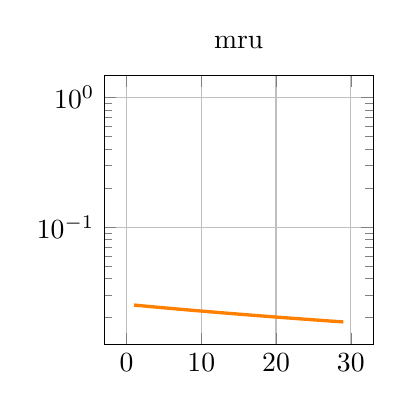
\begin{tikzpicture}
\begin{axis}[ymode=log, title=mru, height=5cm, width=5cm, grid=major, xmin=({-}3.0), xmax=(33.0), ymin=(0.012427), ymax=(1.490182)]
\addplot[very thick,color=orange] coordinates { (1,0.025) (2,0.024691358024691357) (3,0.024390243902439025) (4,0.024096385542168676) (5,0.023809523809523808) (6,0.023529411764705882) (7,0.023255813953488372) (8,0.022988505747126436) (9,0.022727272727272728) (10,0.02247191011235955) (11,0.022222222222222223) (12,0.02197802197802198) (13,0.021739130434782608) (14,0.021505376344086023) (15,0.02127659574468085) (16,0.021052631578947368) (17,0.020833333333333332) (18,0.020618556701030927) (19,0.02040816326530612) (20,0.020202020202020204) (21,0.02) (22,0.019801980198019802) (23,0.0196078431372549) (24,0.019417475728155338) (25,0.019230769230769232) (26,0.01904761904761905) (27,0.018867924528301886) (28,0.018691588785046728) (29,0.018518518518518517)
};


\end{axis}
\end{tikzpicture}
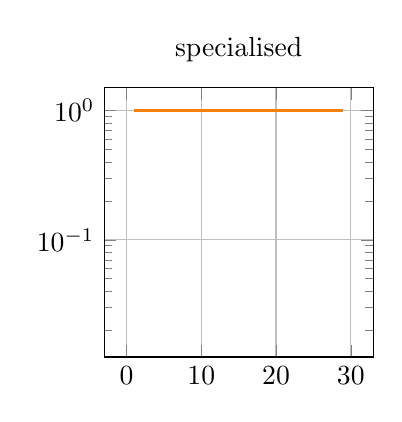
\begin{tikzpicture}
\begin{axis}[ymode=log, title=specialised, height=5cm, width=5cm, grid=major, xmin=({-}3.0), xmax=(33.0), ymin=(0.012427), ymax=(1.490182)]
\addplot[very thick,color=orange] coordinates { (1,1.0) (2,1.0) (3,1.0) (4,1.0) (5,1.0) (6,1.0) (7,1.0) (8,1.0) (9,1.0) (10,1.0) (11,1.0) (12,1.0) (13,1.0) (14,1.0) (15,1.0) (16,1.0) (17,1.0) (18,1.0) (19,1.0) (20,1.0) (21,1.0) (22,1.0) (23,1.0) (24,1.0) (25,1.0) (26,1.0) (27,1.0) (28,1.0) (29,1.0)
};


\end{axis}
\end{tikzpicture}


\end{document}
